\documentclass[12pt]{article}
%\usepackage[document]{ragged2e}
\usepackage{array, amssymb, amsthm, linguex, enumerate, amsmath, physics, enumitem, xcolor, graphicx, xparse}
\let\fg\undefined %remove linguex/siunitx naming clash
\usepackage[english]{babel}
\usepackage[letterpaper,top=2cm,bottom=2cm,left=3cm,right=3cm,marginparwidth=1.75cm]{geometry}
\usepackage[colorlinks=true, allcolors=blue]{hyperref}
\usepackage[group-separator={,}]{siunitx} %\num{12345} -> "12,345"
\usepackage{fancyhdr}
\usepackage{notomath}
\usepackage[T1]{fontenc}
\usepackage{multicol}
\usepackage{mathtools}

%Number sets
\newcommand{\R}{\mathbb{R}}
\newcommand{\C}{\mathbb{C}}
\newcommand{\N}{\mathbb{N}}
\newcommand{\F}{\mathbb{F}}
\renewcommand{\Re}{\operatorname{Re}}
\renewcommand{\Im}{\operatorname{Im}}
\renewcommand{\L}[1]{\mathcal{L}\left({#1}\right)} %Linear Map

\newcommand{\pmp}{\,\pm\,} %add small extra space to \pm

\NewDocumentCommand{\ceil}{ s m }{% ceiling brackets
    \IfBooleanTF{#1}%
    {\lceil #2 \rceil}% starred: no-autosizing
    {\left\lceil #2 \right\rceil}% unstarred: autosizing
}

\NewDocumentCommand{\ceiling}{ s m }{% ceiling brackets
    \IfBooleanTF{#1}%
    {\lceil #2 \rceil}% starred: no-autosizing
    {\left\lceil #2 \right\rceil}% unstarred: autosizing
}

\NewDocumentCommand{\floor}{ s m }{% floor brackets
    \IfBooleanTF{#1}%
    {\lfloor #2 \rfloor}% starred: no-autosizing
    {\left\lfloor #2 \right\rfloor}% unstarred: autosizing
}

\NewDocumentCommand{\pars}{ s m }{% parenthesis
    \IfBooleanTF{#1}%
    {( #2 ) }% starred: no-autosizing
    {\left( #2 \right) }% unstarred: autosizing
}

\NewDocumentCommand{\inner}{ s m }{% inner product
    \IfBooleanTF{#1}%
    {\langle #2 \rangle}% starred: no-autosizing
    {\left\langle #2 \right\rangle}% unstarred: autosizing
}

\NewDocumentCommand{\innerconj}{ s m }{% inner product
    \IfBooleanTF{#1}%
    {\overline{\langle #2 \rangle}}% starred: no-autosizing
    {\overline{\left\langle #2 \right\rangle}}% unstarred: autosizing
}

\NewDocumentCommand{\brac}{ s m }{% brackets
    \IfBooleanTF{#1}%
    {[#2] }% starred: no-autosizing
    {\left[ #2 \right] }% unstarred: autosizing
}

%default latex bracket size naming
\newcommand{\biggbrac}[1]{\bigg[ {#1} \bigg] }
\newcommand{\bigbrac}[1]{\big[ {#1} \big] }
\newcommand{\Bigbrac}[1]{\Big[ {#1} \Big] }


\RenewDocumentCommand{\over}{ s m }{% fraction 1/arg
    \IfBooleanTF{#1}%
    {\dfrac{1}{#2}}% starred: dfrac
    {\frac{1}{#2}}% unstarred: normal frac
}

\NewDocumentCommand{\pover}{ s m }{% parenthesis around fraction (1/arg)
    \IfBooleanTF{#1}%
    {\left(\dfrac{1}{#2}\right)}% starred: dfrac
    {\left(\frac{1}{#2}\right)}% unstarred: normal frac
}

\NewDocumentCommand{\pfrac}{ s m m}{% parenthesis around fraction (arg1/arg2)
    \IfBooleanTF{#1}%
    {\left( \dfrac{{#2}}{{#3}} \right)}% starred: dfrac
    {\left( \frac{{#2}}{{#3}} \right)}% unstarred: normal frac
}


\newcommand{\Xbar}{\bar{X}}
\newcommand{\Ybar}{\bar{Y}}
\newcommand{\xbar}{\bar{x}}
\newcommand{\ybar}{\bar{y}}

\newcommand{\symint}[1]{\int_{- #1}^{#1}}

\newcommand{\limn}{\lim_{n\to\infty}}

\newcommand{\sumn}[1]{\sum_{n=#1}^{\infty}}

\newcommand{\nptl}{\frac{n \pi t}{L}}
\newcommand{\npt}{n \pi t}
\newcommand{\npto}[1]{\frac{n \pi t}{#1}}

\newcommand{\npxl}{\frac{n \pi x}{L}}
\newcommand{\bnxl}{\frac{\beta_n x}{L}}
\newcommand{\npx}{n \pi x}
\newcommand{\np}{n \pi}
\newcommand{\npxo}[1]{\frac{n \pi x}{#1}}
\newcommand{\onp}[1]{\frac{#1}{n \pi}}
\newcommand{\onps}[1]{\frac{#1}{n^2 \pi^2}}
\newcommand{\onpc}[1]{\frac{#1}{n^3 \pi^3}}
\newcommand{\npo}[1]{\frac{n \pi}{#1}}
\newcommand{\cosp}[1]{\cos \pars{#1}}
\newcommand{\sinp}[1]{\sin \pars{#1}}
\newcommand{\intll}{\int_{-L}^{L}}
\newcommand{\intl}{\int_{0}^L}

\newcommand{\gammaDist}[2]{\operatorname{Gamma} \left( {#1},{#2} \right)} %gamma distribution
\NewDocumentCommand{\normalDist}{s g g}{ %normal distibution
    \IfBooleanTF{#1} { % starred, no autosizing parenthesis
      \IfNoValueTF{#2}{
          N (\mu,\, \sigma^2 ) %\normalDist* "default" normal distribution N(\mu, \sigma^2)
        } {
            \IfNoValueTF{#3}{N (#2)}{} %\normalDist{arg} --> N(arg)
        }
      \IfNoValueTF{#3}{}{N ( #2, #3 )}  %\normalDist*{arg1}{arg2} --> N(arg1,arg2)
    }  % else (unstarred) autosize parenthesis
    {
        \IfNoValueTF{#2}{
            N \left(\mu,\, \sigma^2 \right) %\normalDist "default" normal distribution N(\mu, \sigma^2)
        } {
            \IfNoValueTF{#3}{N \left(#2\right)}{} %\normalDist{arg} --> N(arg)
        }
        \IfNoValueTF{#3}{}{N \left( #2, #3 \right)} %\normalDist{arg1}{arg2} --> N(arg1,arg2)
    }
}



%colors
\definecolor{ggreen}{RGB}{0, 127, 0}
\definecolor{dgray}{RGB}{63,63,63}
\definecolor{neonorange}{RGB}{255,47,0}
\definecolor{mygray}{rgb}{0.5,0.5,0.5}
\definecolor{eblue}{RGB}{0,74,127}
\newcommand{\red}[1]{\color{red}{#1}\color{black}}
\newcommand{\green}[1]{\color{ggreen}{#1}\color{black}}
\newcommand{\blue}[1]{\color{blue}{#1}\color{black}}
\newcommand{\setRed}{\color{red}}
\newcommand{\setBlack}{\color{black}}
\newcommand{\setBlue}{\color{blue}}
\newcommand{\setGreen}{\color{ggreen}}

\newcommand{\coshp}[1]{\cosh \pars{#1}}
\newcommand{\sinhp}[1]{\sinh \pars{#1}}
\newcommand{\cunt}{\frac{c n \pi t}{L}}
\newcommand{\absl}{\abs{\lambda}}
\newcommand{\rabsl}{\sqrt{\abs{\lambda}}}
\newcommand{\qiffq}{\quad\iff\quad}
\newcommand{\thru}[1]{{#1}_1, \dots, {#1}_n}
\newcommand{\sumThru}[1]{{#1}_1 + \cdots + {#1}_n}
\newcommand{\yn}{Y_1, \dots, Y_n} % Y_1, ..., Y_n
\newcommand{\xn}{X_1, \dots, X_n} % Y_1, ..., Y_n

%hats and tildes
\newcommand{\that}{\widehat{\theta}} % theta hat
\newcommand{\phat}{\widehat{p}} % p hat
\newcommand{\qhat}{\widehat{q}} % p hat
\newcommand{\psihat}{\widehat{\psi}} % psi hat
\newcommand{\Psihat}{\widehat{\Psi}} % Psi hat
\newcommand{\ptilde}{\widetilde{p}} % psi tilde
\newcommand{\Psitil}{\widetilde{\Psi}} % Psi tilde
\newcommand{\betah}{\widehat{\beta}} % beta hat

%2x2 matrix shortcuts
\newcommand{\detx}[4]{\begin{vmatrix}{#1} & {#2}\\{#3}&{#4}\end{vmatrix}} % 2x2 determinant
\newcommand{\dety}[9]{\begin{vmatrix}{#1} & {#2} & {#3} \\{#4}&{#5}&{#6}\\ {#7} & {#8} & {#9}\end{vmatrix}} % 3x3 determinant
\newcommand{\bmaty}[9]{\begin{bmatrix}{#1} & {#2} & {#3} \\{#4}&{#5}&{#6}\\ {#7} & {#8} & {#9}\end{bmatrix}} % 3x3 matrix
\newcommand{\bmat}[4]{\begin{bmatrix}{#1} & {#2}\\{#3}&{#4}\end{bmatrix}} % 2x2 matrix brackets
\renewcommand{\pmat}[4]{\begin{pmatrix}{#1} & {#2}\\{#3}&{#4}\end{pmatrix}} % 2x2 matrix parenthesis

%remove any enumerate/itemize indent temporarily
\makeatletter   %% <- make @ usable in macro names
\newcommand*\notab[1]{%
  \begingroup   %% <- limit scope of the following changes
    \par        %% <- start a new paragraph
    \@totalleftmargin=0pt \linewidth=\columnwidth
    %% ^^ let other commands know that the margins have been reset
    \parshape 0
    %% ^^ reset the margins
    #1\par      %% <- insert #1 and end this paragraph
  \endgroup
}
\makeatother    %% <- revert @


\newcommand{\dimrange}[1]{\operatorname{dim}\operatorname{range}{#1}} % dimrange
\newcommand{\dimnull}[1]{\operatorname{dim}\operatorname{null}{#1}} % dimnull
\newcommand{\range}[1]{\operatorname{range}{#1}} %range
\newcommand{\nullspace}{\operatorname{null}} %null

% polynomial notation
\NewDocumentCommand{\poly}{ s g g }{%
    \IfBooleanTF{#1} {
        \IfNoValueTF{#2} {
            \mathcal{P}(\mathbb{R})
        } {
            \mathcal{P}_{#2}(\mathbb{R})
        }
    } {
        \IfNoValueTF{#3} {
            {\mathcal{P}(#2)}
        } { %else
            {\mathcal{P}_{#2}(#3)}
        }
    }
}

\NewDocumentCommand{\bias}{ s m }{% bias(arg)
    \IfBooleanTF{#1}%
    {\operatorname{bias}(#2)}% starred: no autosizing
    {\operatorname{bias}\left(#2\right)}% unstarred: autosizing
}

\NewDocumentCommand{\MSE}{ s m }{% MSE(arg)
    \IfBooleanTF{#1}%
    {\operatorname{MSE}(#2)}% starred: no autosizing
    {\operatorname{MSE}\left(#2\right)}% unstarred: autosizing
}

\NewDocumentCommand{\Var}{ s m }{% variance with parenthesis V(arg)
    \IfBooleanTF{#1}%
    {\operatorname{Var}(#2)}% starred: no autosizing
    {\operatorname{Var}\left(#2\right)}% unstarred: autosizing
}

\NewDocumentCommand{\Varb}{ s m }{% variance with brackets V[arg]
    \IfBooleanTF{#1}%
    {\operatorname{Var}[\,#2\,]}% starred: no autosizing
    {\operatorname{Var}\left[\,#2\,\right]}% unstarred: has autosizing
}

\NewDocumentCommand{\Vb}{ s m }{% another renaming of variance with brackets V[arg]
    \IfBooleanTF{#1}%
    {\operatorname{Var}[\,#2\,]}% starred: no autosizing
    {\operatorname{Var}\left[\,#2\,\right]}% unstarred: has autosizing
}

\NewDocumentCommand{\E}{ s m }{% expectation with parenthesis E(arg)
    \IfBooleanTF{#1}%
    {\operatorname{E}(#2)}% starred: no autosizing
    {\operatorname{E}\left(#2\right)}% unstarred: has autosizing
}

\NewDocumentCommand{\Eb}{ s m }{% expectation with brackets E[arg]
    \IfBooleanTF{#1}%
    {\operatorname{E}[#2]}% starred: no autosizing
    {\operatorname{E}\left[#2\right]}% unstarred: has autosizing
}

\RenewDocumentCommand{\P}{ s m }{% probability with parenthesis Pr(arg)
    \IfBooleanTF{#1}%
    {\Pr (#2) }% starred: no autosizing
    {\Pr \left( #2 \right) }% unstarred: has autosizing
}

\NewDocumentCommand{\prob}{ s m }{% probability with parenthesis Pr(arg)
    \IfBooleanTF{#1}%
    {\Pr (#2) }% starred: no autosizing
    {\Pr \left( #2 \right) }% unstarred: has autosizing
}

\NewDocumentCommand{\eff}{ s m }{% efficiency with parenthesis eff(arg)
    \IfBooleanTF{#1}%
    {\operatorname{eff}(#2)}% starred: no autosizing
    {\operatorname{eff}\left(#2\right)}% unstarred: has autosizing
}

%vertical vector of up to 8 elements
\NewDocumentCommand\vvec{s m g g g g g g g}{%
    \IfBooleanTF{#1} {
        \begin{bmatrix}% if starred use brackets
            \IfNoValueTF{#2}{}{#2}
            \IfNoValueTF{#3}{}{\\#3}
            \IfNoValueTF{#4}{}{\\#4}
            \IfNoValueTF{#5}{}{\\#5}
            \IfNoValueTF{#6}{}{\\#6}
            \IfNoValueTF{#7}{}{\\#7}
            \IfNoValueTF{#8}{}{\\#8}
        \end{bmatrix}
    }  % else (unstarred) use parethesis
    {
        \begin{pmatrix}%
            \IfNoValueTF{#2}{}{#2}
            \IfNoValueTF{#3}{}{\\#3}
            \IfNoValueTF{#4}{}{\\#4}
            \IfNoValueTF{#5}{}{\\#5}
            \IfNoValueTF{#6}{}{\\#6}
            \IfNoValueTF{#7}{}{\\#7}
            \IfNoValueTF{#8}{}{\\#8}
        \end{pmatrix}
    }
}
\def\Cov{\operatorname{Cov}} %Covariance
\def\df{\text{df}} %degrees of freedom

\NewDocumentCommand{\example}{ s g }{% Example header
    \IfBooleanTF{#1}%
    {\vspace{0.1in}}% starred: 0.1in
    {\vspace{0.2in}}% unstarred: 0.2in
    \IfNoValueTF{#2} {\noindent\textbf{\color{eblue} Example: }}{\noindent\textbf{\color{eblue} Example (#2): }}
}
\NewDocumentCommand{\disc}{ s }{% Discussion header
    \IfBooleanTF{#1}%
    {\vspace{0.1in}\noindent\textbf{Discussion: } }% starred: 0.1in
    {\vspace{0.2in}\noindent\textbf{Discussion: } }% unstarred: 0.2in
}
\NewDocumentCommand{\defn}{ s }{% Definition header
    \IfBooleanTF{#1}%
    {\vspace{0.1in}\noindent\textbf{\color{neonorange} Definition: } }% starred: 0.1in
    {\vspace{0.2in}\noindent\textbf{\color{neonorange} Definition: } }% unstarred: 0.2in
}
\NewDocumentCommand{\reason}{ s }{% Reason header
    \IfBooleanTF{#1}%
    {\vspace{0.1in}\noindent\textbf{Reason:} }% starred: 0.1in
    {\vspace{0.2in}\noindent\textbf{Reason:} }% unstarred: 0.2in
}
\NewDocumentCommand{\recall}{ s }{% Recall header
    \IfBooleanTF{#1}%
    {\vspace{0.1in}\noindent\textit{Recall:} }% starred: 0.1in
    {\vspace{0.2in}\noindent\textit{Recall:} }% unstarred: 0.2in
}
\NewDocumentCommand{\remark}{ s }{% Remark header
    \IfBooleanTF{#1}%
    {\vspace{0.1in}\noindent\textit{Remark:} }% starred: 0.1in
    {\vspace{0.2in}\noindent\textit{Remark:} }% unstarred: 0.2in
}

\NewDocumentCommand{\soln}{ s }{% Remark header
    \IfBooleanTF{#1}%
    {\vspace{0.1in}\noindent\textbf{Solution: } }% starred: 0.1in
    {\vspace{0.2in}\noindent\textbf{Solution: } }% unstarred: 0.2in
}

\newcommand{\proj}[2]{\operatorname{proj}_{{#1}}{#2}} %projection
\newcommand{\wideand}{\qquad \text{and} \qquad}

\newcommand{\bu}[1]{\textbf{\underline{{#1}}} } %bold underline
\newcommand{\boldit}[1]{\textbf{\textit{{#1}}} } %bold italix

% put actual quotation marks "around something"
\newcommand{\say}[1]{\textquotedblleft{#1}\textquotedblright}

% max{arg} and min{arg}
\renewcommand{\max}[1]{\operatorname{max}\left\{ #1 \right\}}
\renewcommand{\min}[1]{\operatorname{min}\left\{ #1 \right\}}

\newcommand{\Span}[1]{\operatorname{span}\left\{ #1 \right\}}

%Create a new vspace line no indent
\newcommand{\nl}{\vspace{0.1in}\noindent}
\newcommand{\nnl}{\vspace{0.2in}\noindent}
\newcommand{\nnnl}{\vspace{0.3in}\noindent}
\textwidth=7.02in
\hoffset=-.425in

\setcounter{MaxMatrixCols}{20}
\begin{document}
\pagestyle{fancy}
\fancyhf{}
\fancyhead[RO]{Matthew Wilder}
\fancyhead[LO]{MTH 427 - Homework \#6}
\fancyfoot[CO]{Page \thepage}

\noindent MTH 427 - Spring 2023
\\Assignment \#6
\\Due: Friday, 4 7 2023

\textbf{Problem 1.2 (a, b)}
\begin{enumerate}[label=(\alph*)]
    \item  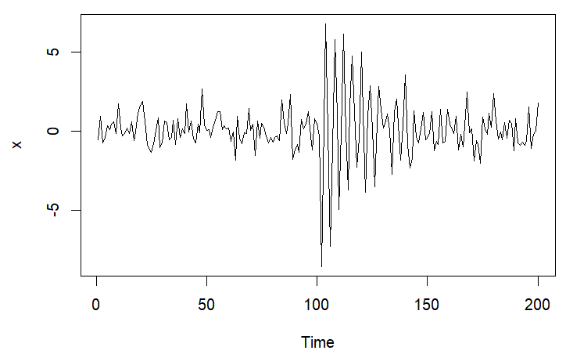
\includegraphics[width=6in]{img/a.PNG}
    \item  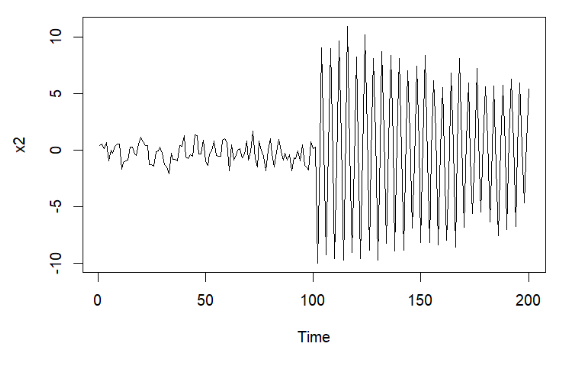
\includegraphics[width=6in]{img/b.PNG}
\end{enumerate}

\textbf{Problem 1.4 (a,b)}
\begin{align*}
    \gamma(s, t) &= \Cov(x_s, x_t)\\ &= \Eb{(x_s - \mu_s)(x_t - \mu_t)}\\
    &= \Eb{x_s x_t - x_s \mu_t - \mu_s x_t + \mu_t \mu_s}\\
    &= \Eb{x_s x_t} - \Eb{x_s \mu_t} - \Eb{\mu_s x_t} + \Eb{\mu_t \mu_s}\\
    &= \Eb{x_s x_t} -\mu_t \Eb{x_s} - \mu_s \Eb{x_t} + \mu_t \mu_s\\
    &= \Eb{x_s x_t} -\mu_t \mu_s - \mu_s \mu_t + \mu_t \mu_s\\
    &= \Eb{x_s x_t} -\mu_s \mu_t
\end{align*}

\textbf{Problem 1.6 (a, b)}
\begin{enumerate}[label=(\alph*)]
    \item $\Eb{x_t} = \Eb{\beta_1} + \Eb{\beta_2 t} + \Eb{w_t} = \beta_1 + \beta_2 t  + 0$. Since this is dependent on $t$, it is non-stationary.
    \item Need to show 2 conditions. First, $\Eb{x_t}$ is constant, and second $\gamma(t+h, \; t)$ depends only on $h$. \begin{enumerate}[label=(\arabic*)]
        \item \begin{align*}
            \Eb{y_t} &= \Eb{x_t - x_{t-1}}\\
            &= \Eb{x_t} - \Eb{x_{t-1}}\\
            &=  \beta_1 + \beta_2 t - \brac{ \beta_1 + \beta_2 (t-1)}\\
            &= \beta_2 \tag{Constant}
        \end{align*}
        \item $y_t = x_t - x_{t-1}$ and $x_t = \beta_1 + \beta_2 t + w_t$ \begin{align*}
            & \gamma(t+h, \; t)
            \\ &= \Cov(y_{t+h},\; y_t)
            \\ &= \Cov(x_{t+h} - x_{t+h-1},\; x_t - x_{t-1})\\
            % &= \Cov(x_{t+h},\; x_t) + \Cov(x_{t+h},\; - x_{t-1})
            % + \Cov(- x_{t+h-1},\; x_t) + \Cov(- x_{t+h-1},\; - x_{t-1})\\
            &= \Cov(\beta_2 (t+h) + w_{t+h} \; - \; (\beta_2 (t+h-1) + w_{t+h-1} ), \quad \beta_2 (t) + w_{t} \; - \; (\beta_2 (t-1) + w_{t-1} )) \\
            &= \Cov(w_{t+h} + w_{t+h-1},\; w_t + w_{t-1})\\
            &= \Cov(w_{t+h},\; w_t) +  \Cov(w_{t+h},\; w_{t-1}) +  \Cov(w_{t+h-1},\; w_t) +  \Cov(w_{t+h-1},\; w_{t-1})
        \end{align*}
        If $h = 0$ then $$\gamma(t+0,\; t) = \underbrace{\Cov(w_{t},\; w_t)}_{\sigma_w^{2}} +
         \underbrace{\Cov(w_{t},\; w_{t-1})}_{0} +  \underbrace{\Cov(w_{t-1},\; w_t)}_{0} +  \underbrace{\Cov(w_{t-1},\; w_{t-1})}_{\sigma_w^{2}} = 2\sigma_w^2$$
         If $h = \pm 1$ then $$\gamma(t+1,\; t) = \underbrace{\Cov(w_{t+1},\; w_t)}_{0} +
         \underbrace{\Cov(w_{t+1},\; w_{t-1})}_{0} +  \underbrace{\Cov(w_{t},\; w_t)}_{\sigma_w^{2}} +  \underbrace{\Cov(w_{t},\; w_{t-1})}_{0} = \sigma_w^2$$
        If $h = \pm 2$ then $$\gamma(t+2, \; t) = \Cov(w_{t+2} + w_{t+1},\; w_t + w_{t-1}) = 0$$
        Similarly for $\abs{h} > 2,\; \gamma(t+h, t) \equiv 0$. 
        \\In none of these cases does $\gamma$ depend on $t$. 
    \end{enumerate}
\end{enumerate}

\newpage 
\textbf{1.8 (a,b,c)}
\begin{enumerate}[label=(\alph*)]
    \item \begin{align*}
        x_t &= \delta + w_t + x_{t_1}\\
        &= \delta+w_t + \delta + w_{t-1} + x_{t-2}\\
        &\;\,\vdots \\
        &= (\delta + w_t) + (\delta + w_{t-1}) + \dots + (\delta + w_1) + \underbrace{x_0}_{0}\\
        &= \sum_{n=1}^t (\delta + w_n) \\
        &= t \delta + \sum_{n=1}^t w_n
    \end{align*}
    \item \begin{align*}
        \Eb{x_t} &= \Eb{ t \delta + \sum_{n=1}^t w_n}\\
        &= t \delta +  \sum_{n=1}^t\Eb{ w_n} \\
        &= t \delta + \sum_{n=1}^t 0\\
        &= t \delta
    \end{align*}
    And the ACVF is $t \sigma_w^2$ by the recursive nature.
    \item It is non stationary because the mean isnt constant and the ACVF depends on t.
\end{enumerate}
\newpage
\textbf{2.1 Exercise 1}

\noindent 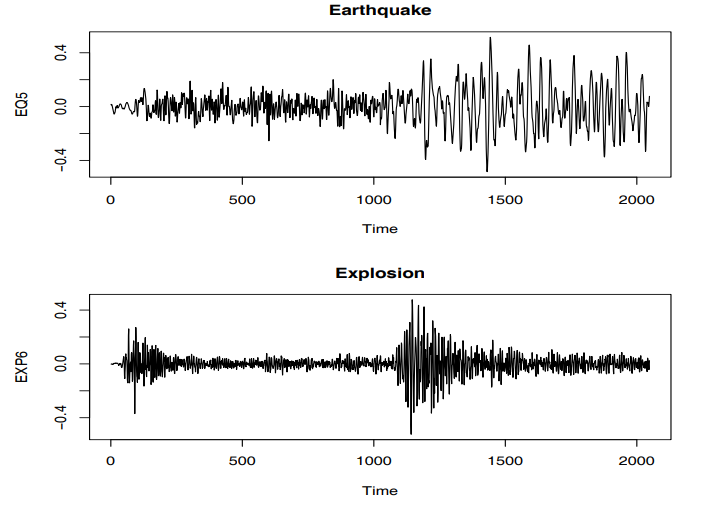
\includegraphics[width=6in]{img/17.PNG}

\noindent 1.2a looks like the explosion, where it quickly decays near 0, and 1.2b looks like the earthquake where it slowly decays back near 0.

\textbf{2.2 Exercise 2}
\begin{enumerate}[label=(\alph*)]
    \item \textbf{Accidental deaths in USA:} Not stationary because the value depends on $t$. (More deaths when t=July and less deaths when t=Feb)
    \item \textbf{USA population} Not stationary because it grows in time.
    \item \textbf{International Airline Passengers} Not stationary because it depends on the time of year, as well as growing linearly.
\end{enumerate}


\textbf{2.3 Exercise 3}
\begin{enumerate}[label=(\alph*)]
    \item $\Eb{X_t} = \Eb{W_2} = \mu = 0$ constant therefore stationary (with mean 0).\\Then $\gamma(t+h, t) = \Cov(X_{t+h}, X_{t}) = \Cov(W_2, W_2) = \Varb{W_2} = \sigma^2 = 1$
    \item $\Eb{X_t} = \Eb{t} + \Eb{W_2} = \Eb{t}$ depends on t, not stationary
    \item Since $\Varb{X} = \Eb{X^2} - \Eb{X}^2$ then $\Eb{X^2} = \Varb{X} + \Eb{X}^2 = \Cov(X, X)+ \Eb{X}^2$. It follows that $\Eb{X_t} = \Eb{W_t^2} = \Cov(W_t, W_t) + \Eb{W_t}^2 = \sigma^2 + \mu^2 = 1 + 0^2 = 1$. Stationary because constant value. \\Then $\gamma(h) = \Eb{(W_{t+h}^2 - \mu) (W_{t}^2 - \mu)} = \Eb{W_{t+h}^2W_t^2}$. Then $\gamma(0) = \Eb{W_t^2 W_t^2} = \Eb{W_t^4}$. Letting $Z := W_t^2$, then $\gamma(h) = \Eb{Z^2} = \Varb{Z} + \Eb{Z}^2$. Using how we computed the mean, $\Eb{Z}^2 = \Eb{W_{t}^2}^2 = 1^1 = 1$. For the variance, this is chi-square with 1 degree of freedom. Then by properties of chi-square, $\Varb{Z} = 2$. Thus $\gamma(0) = \Eb{W_t^4 } = \Eb{Z^2} = 2+1 = 3$. For $h \neq 0$ then $W_{t+h^{\ast}}$ and $W_{t}$ and independent so for $h^{\ast} \in \R^{\ast}$ then $\gamma(h^{\ast}) = \Eb{W_{t+h^{\ast}}^2} \Eb{W_{t}^2} = 1 \cdot 1 = 1$
\end{enumerate}


\end{document}
